\documentclass[12pt, letterpaper]{article}
\usepackage[titletoc,title]{appendix}
\usepackage{color}
\usepackage{booktabs}
\usepackage[usenames,dvipsnames,svgnames,table]{xcolor}
\definecolor{dark-red}{rgb}{0.75,0.10,0.10}
\definecolor{bluish}{rgb}{0.05,0.05,0.85}
\PassOptionsToPackage{unicode}{hyperref}
\PassOptionsToPackage{naturalnames}{hyperref}
\usepackage[margin=1in]{geometry}
\usepackage[linkcolor=blue,
			colorlinks=true,
			urlcolor=blue,
			pdfstartview={XYZ null null 1.00},
			pdfpagemode=UseNone,
			citecolor={bluish},
			pdftitle={partisan}]{hyperref}

%\newcites{SI}{SI References}
\usepackage{natbib}

\usepackage{float}

\usepackage{geometry}  % see geometry.pdf on how to lay out the page. There's lots.
\geometry{letterpaper} % This is 8.5x11 paper. Options are a4paper or a5paper or other...
\usepackage{graphicx}  % Handles inclusion of major graphics formats and allows use of
\usepackage{amsfonts,amssymb,amsbsy}
\usepackage{amsxtra}
\usepackage{verbatim}
%\setcitestyle{round,semicolon,aysep={},yysep={;}}
\usepackage{setspace} % Permits line spacing control. Options are:
%\doublespacing
%\onehalfspace
%\usepackage{sectsty}    % Permits control of section header styles
\usepackage{pdflscape}
\usepackage{fancyhdr}   % Permits header customization. See header section below.
\usepackage{url}        % Correctly formats URLs with the \url{} tag
\usepackage{fullpage}   %1-inch margins
\usepackage{multirow}
\usepackage{verbatim}
\usepackage{rotating}
\setlength{\parindent}{3em}

%\usepackage[T1]{fontenc}
%\usepackage[bitstream-charter]{mathdesign}

\usepackage{chngcntr}
\usepackage{longtable}
\usepackage{adjustbox}
\usepackage{dcolumn}

\usepackage[nameinlink, capitalize, noabbrev]{cleveref}

\def\citeapos#1{\citeauthor{#1}'s (\citeyear{#1})}

\makeatother

\usepackage{footmisc}
\setlength{\footnotesep}{\baselineskip}
\makeatother
\renewcommand{\footnotelayout}{\normalsize \doublespacing}


% Colors
\usepackage{color}

\newcommand{\bch}{\color{blue}\em  }   % begin change
\newcommand{\ying} {\color{orange}\em  }   % begin change
\newcommand{\bgcd} {\color{purple}\em }
\newcommand{\ech}{\color{black}\rm  }    % end change

% Caption
\usepackage[hang, font=small,skip=0pt, labelfont={bf}]{caption}
%\captionsetup[subtable]{font=small,skip=0pt}
\usepackage{subcaption}

% tt font issues
% \renewcommand*{\ttdefault}{qcr}
\renewcommand{\ttdefault}{pcr}


\setcounter{page}{0}

\usepackage{lscape}
\renewcommand{\textfraction}{0}
\renewcommand{\topfraction}{0.95}
\renewcommand{\bottomfraction}{0.95}
\renewcommand{\floatpagefraction}{0.40}
\setcounter{totalnumber}{5}
\makeatletter
\providecommand\phantomcaption{\caption@refstepcounter\@captype}
\makeatother


\title{\Large{Holier Than Thou: Partisan Gap in Consumption\\ of Pornography Online}\footnote{You can download the replication materials from \href{http://github.com/soodoku/adult}{https://github.com/soodoku/adult}}}

\author{Lucas Shen\thanks{Lucas is a Research Fellow at Asia Competitiveness Institute, Lee Kuan Yew School of Public Policy, at the National University of Singapore, \href{mailto:lucas@lucasshen.com}{\footnotesize{\texttt{lucas@lucasshen.com}}}} \and Gaurav Sood\thanks{Gaurav can be reached at \href{mailto:gsood07@gmail.com}{\footnotesize{\texttt{gsood07@gmail.com}}}}\vspace{.5cm}}

\date{\today}

\begin{document}
\maketitle

\begin{comment}

setwd("Documents/Github/adult/ms/")
tools::texi2dvi("porn.tex", pdf=TRUE, clean=TRUE) 
setwd(basedir)

\end{comment}

\begin{abstract}
\noindent Consumption of pornography has been blamed for a variety of societal ills, including the rise in misogyny, sex crimes, and the coarsening of culture. Using passively collected browsing data from YouGov, we investigate how much pornography Americans consume online. We find that there is a sharp positive skew in the consumption of pornography, with a small number of users consuming lots of pornography and most consuming small amounts. The median American Internet user today spends X minutes per month consuming pornography, visiting Y sites per month; the 95th percentile is X and Y respectively. Lastly, we find that, unlike previous research \citep{macinnis2015american, edelman2009markets}, which relied on ecological inference, Democrats consume slightly more pornography than Republicans.
\end{abstract} 
\clearpage
\doublespace

Consumption of pornography is associated with a variety of disturbing attitudes, beliefs, emotions, and behaviors. Consuming pornography is associated with support for violence against women \citep{hald2010pornography, malamuth2012pornography, donnerstein1984pornography}, belief in rape myths \citep{foubert2011pornography}, increased gender role conflict, lesser sexual satisfaction \citep{szymanski2014psychological, stewart2012young}, poorer relationship quality \citep{szymanski2014psychological, szymanski2015male}, and sexually risky behaviors such as engaging in paid sex, and having extramarital sex \citep{wright2012internet}. A lot of popular pornography also contains a healthy dose of violence. An analysis of popular pornography revealed that 88.2\% of the scenes contained physical aggression, and 48.7\% verbal aggression \citep{bridges2010aggression}. For all these reasons, there are serious concerns about consumption of pornography.

In this paper, using passive browsing data from YouGov, we investigate how much pornography Americans consume online. We find that there is a sharp skew in the consumption of pornography, with a small set of users consuming a large chunk of pornography. The median American Internet user spends X minutes per month (Y\% of their time online) consuming pornography, visiting Y unique sites; the 95th percentile for time spent consuming pornography online is YY minutes.

We also use the data to shed light on an age-old debate --- whether Democrats consume more pornography than Republicans or vice versa. Both parties claim the higher moral ground. And in surveys both parties think consumption of pornography is abhorrent, plausibly for different reasons. Unlike previous research, which relied on ecological inference, we find that Democrats consume slightly more pornography online than Republicans \citep{macinnis2015american, edelman2009markets}. Adjusting for background covariates like age, gender etc., further mutes the differences.

\section*{Data}
We use passively observed browsing data from a YouGov survey to measure the consumption of adult content. YouGov maintains a large online panel recruited through a variety of methods. It uses matched sampling to survey respondents: The provider first draws a random sample from a large synthetic representative sampling frame, finds respondents that match the sampled individuals from its panel, and invites them to take a survey. For details and validation, see \citet{rivers2009}. For this particular sample, panelists also provided de-identified access to their web browsing activity via passive metering software installed voluntarily on their computers. The software, called RealityMine, can be uninstalled at any point and captures visited web URLs independent of the type of browser or browser-specific privacy settings.\footnote{RealityMine does not save passwords or financial transactions, and personally identifying information is screened out by the survey provider.} At the time this data was made available in June, 2022, YouGov had recruited 1,200 individuals to the web tracking panel, which is currently marketed as YouGov Pulse. The passive metering component of this particular opt-in panel adds a layer of selectivity to the sampling process. 

\section*{Measuring Consumption of Adult Content}
For YouGov, we only observe data from a single machine per person. Our analyses should hold if people exhibit similar consumption patterns across devices. If that is too implausible an assumption, then we must decide on the direction of error and how it affects our analyses. We think it is likely that people would be less likely to search for pornography on machines on which they have installed passive monitoring software (though the data are de-identified). If that is so, our estimates are a lower bound of net consumption of pornography per machine. As the number of devices per person is increasing, all these numbers need to be adjusted. Next, is measurement error correlated with ideology? We have little reason to expect that, but we have no capacity to check if it is true. Thus, for current purposes, we assume that it is so.  

We code pornographic content at the domain level. Our main analysis depends on the domain classifications that come with YouGov data. In the Appendix, we use a keyword classifier and a machine learning classifier. As you will see, all of these methods consistently show the same thing. All of this ignores pornography available via more conventional channels. For instance, some pornography is consumed on sites like Tumblr.

\section*{Results}

Our primary dependent variables of interest are: total time spent on pornographic sites and the proportion of time spent on pornographic sites. (In the appendix, we show similar analysis for visits.) 

\begin{figure}[h]
\centering
\caption{Distribution of Consumption of Pornography Online}
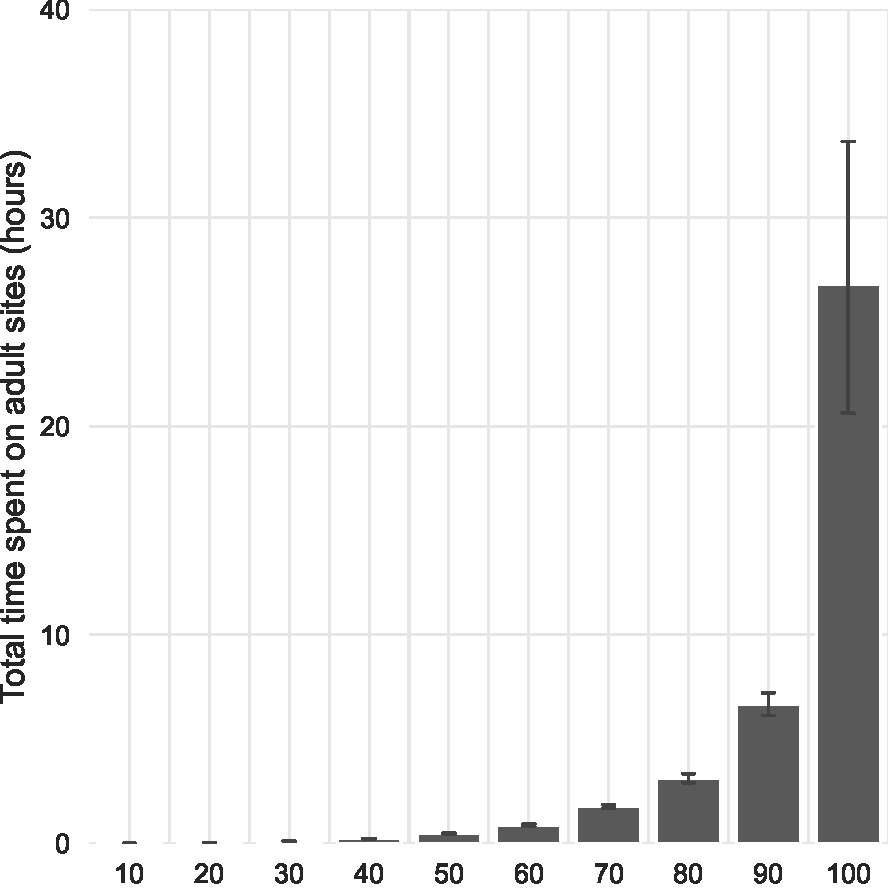
\includegraphics[width=.55\linewidth]{../figs/distribution_duration_on_adultsites.pdf}
\caption*{\footnotesize \emph{Notes:} 
	Hours spent on adult sites by individuals who consumed pornography in the sample period.
	Individuals are split into deciles with each bin containing approximately the same number of individuals.
	Height of bars indicate mean of each bin.
	Capped vertical bars are 95\% confidence intervals.
	See \cref{tab:distribution_duration} for the more tabulated values.
}
\label{fig:distribution_duration}
\end{figure}

\begin{figure}[h]
\centering
\caption{Proportion of Visits to Pornographic Sites}
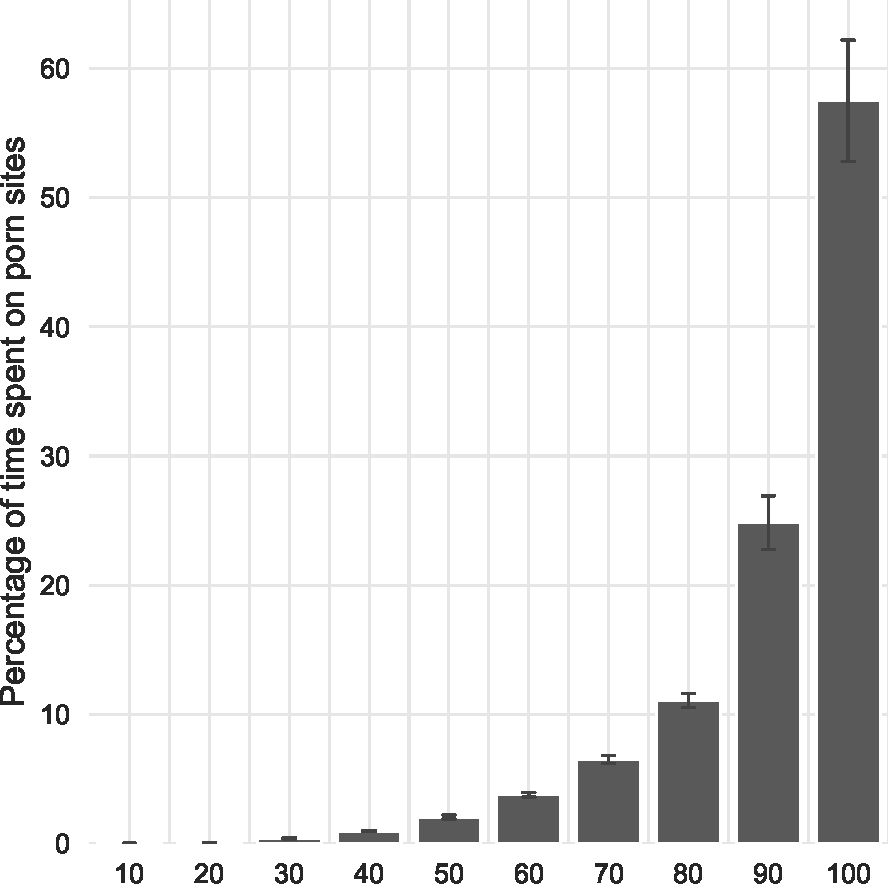
\includegraphics[scale=.75]{../figs/distribution_proportion_duration_on_adultsites.pdf}
\label{fig:distribution_prop_duration}
\end{figure}

\begin{figure}[h]
\centering
\caption{Distribution of Consumption of Pornography Online by Party}
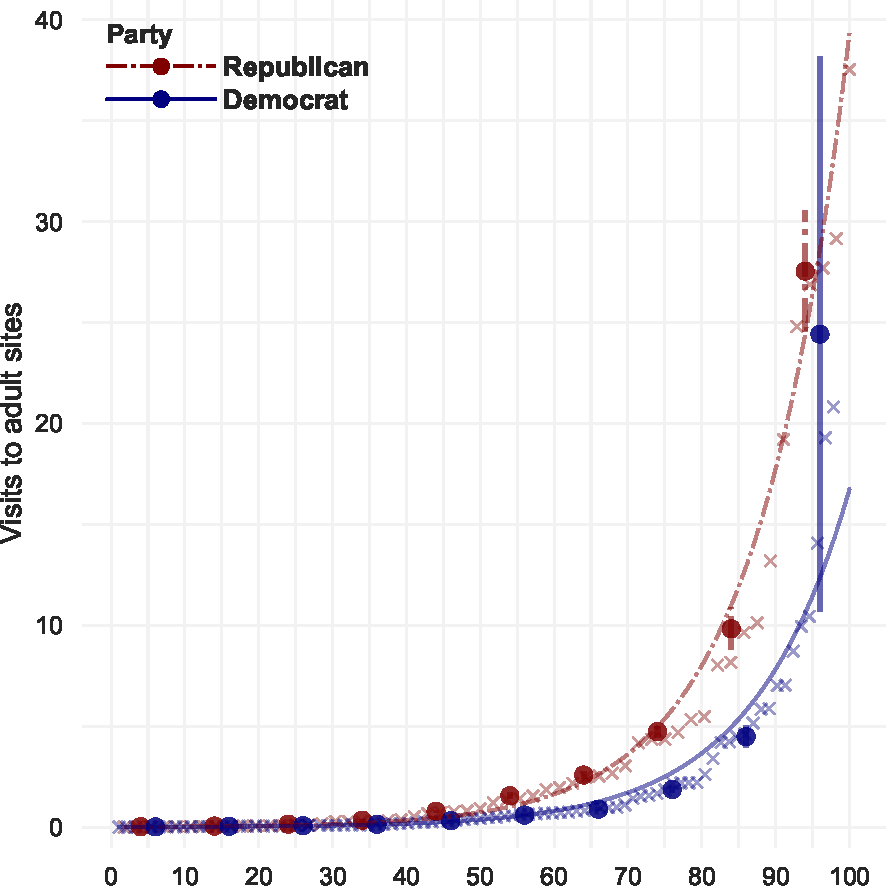
\includegraphics[scale=.75]{../figs/distribution_duration_on_adultsites_by_party.pdf}
\label{fig:distribution_duration_party}
\end{figure}

To formally test for these differences, we ran quantile regression, regressing the duration on party. 

\begin{figure}[h]
\centering
\caption{Distribution of Consumption of Pornography Online by Party}
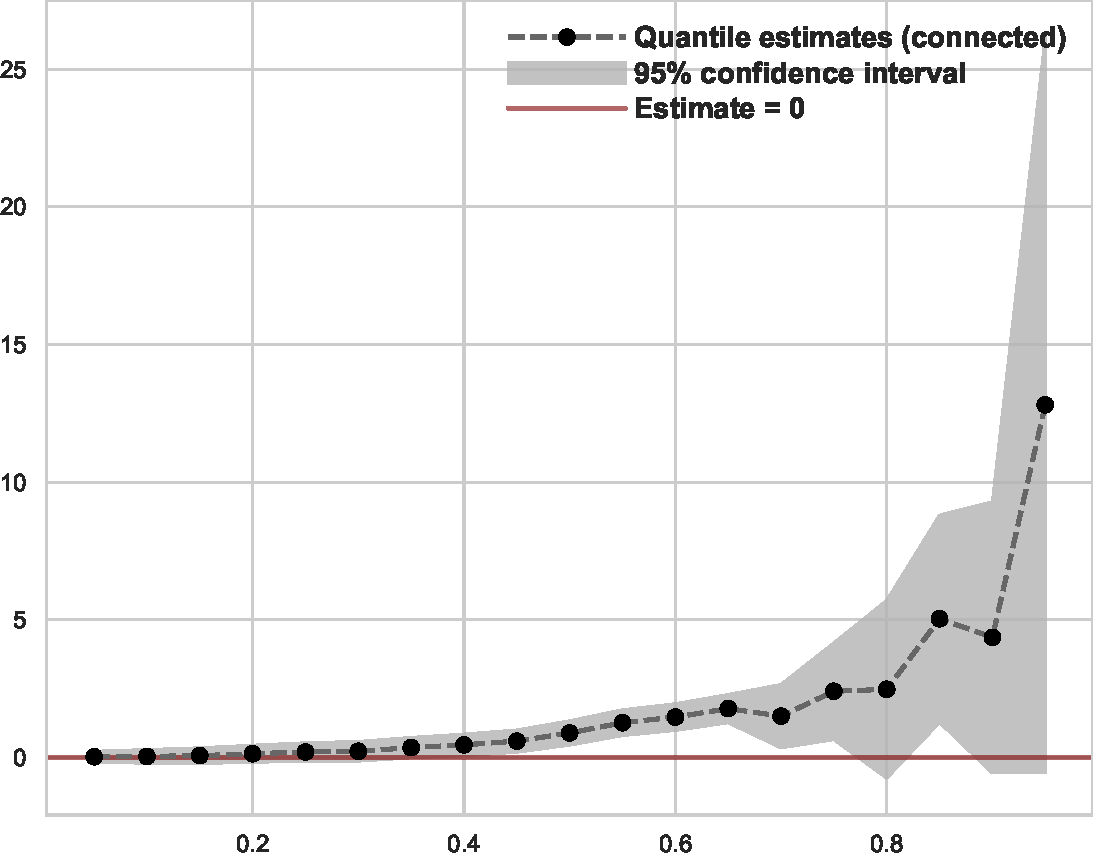
\includegraphics[scale=.75]{../figs/quantile_reg_nonzero_duration_adult.pdf}
\label{fig:quantile_regression_duration}
\end{figure}

These minor differences (or lack of differences) could be because of the demographic differences we see across the party. Next, we control for immutable characteristics like age and gender to see if that adjustment changes the picture much. Given how concentrated pornographic consumption is in our data, it is unlikely to make much of a difference and that is indeed what we find. 


% Table created by stargazer v.5.2 by Marek Hlavac, Harvard University. E-mail: hlavac at fas.harvard.edu
% Date and time: Wed, Mar 30, 2016 - 18:29:29
% Requires LaTeX packages: dcolumn 
\begin{table}[!htbp] \centering 
  \caption{The effect of ideology on four separate dependent variables measuring pornography consumption.} 
  \label{tab:ideomodels} 
\small 
\begin{tabular}{@{\extracolsep{5pt}}lD{.}{.}{-2} D{.}{.}{-2} D{.}{.}{-2} D{.}{.}{-2} } 
\\[-1.8ex]\hline \\[-1.8ex] 
 & \multicolumn{1}{c}{Number of visits} & \multicolumn{1}{c}{Pct. visits} & \multicolumn{1}{c}{Total time (seconds)} & \multicolumn{1}{c}{Pct. time} \\ 
\\[-1.8ex] & \multicolumn{1}{c}{(1)} & \multicolumn{1}{c}{(2)} & \multicolumn{1}{c}{(3)} & \multicolumn{1}{c}{(4)}\\ 
\hline \\[-1.8ex] 
 Ideology: Conservative & -0.60^{*} & 0.001 & -929.60 & 0.001 \\ 
  & (0.33) & (0.004) & (759.29) & (0.004) \\ 
  Ideology: Don't know & -1.02^{**} & -0.005 & -862.56 & 0.001 \\ 
  & (0.44) & (0.01) & (1,068.65) & (0.01) \\ 
  Ideology: Liberal & -0.64^{**} & -0.004 & -1,228.61 & -0.003 \\ 
  & (0.30) & (0.004) & (771.12) & (0.004) \\ 
  Ideology: Very conservative & -0.93^{**} & -0.004 & -1,265.14 & -0.002 \\ 
  & (0.39) & (0.004) & (805.47) & (0.004) \\ 
  Ideology: Very liberal & -0.04 & 0.01^{*} & 1,723.00^{**} & 0.01^{***} \\ 
  & (0.28) & (0.004) & (856.46) & (0.004) \\ 
  Age: 25-44 & -0.55^{**} & -0.004 & -2,024.46^{**} & -0.01^{***} \\ 
  & (0.27) & (0.004) & (885.57) & (0.004) \\ 
  Age: 45-64 & -1.69^{***} & -0.01^{*} & -3,347.91^{***} & -0.01^{***} \\ 
  & (0.35) & (0.004) & (907.86) & (0.004) \\ 
  Age: 65+ & -1.69^{***} & -0.01^{**} & -2,415.55^{**} & -0.01^{***} \\ 
  & (0.41) & (0.005) & (1,035.71) & (0.005) \\ 
  Gender: Male & 2.39^{***} & 0.02^{***} & 3,448.81^{***} & 0.02^{***} \\ 
  & (0.31) & (0.002) & (515.79) & (0.002) \\ 
  Married & -1.31^{***} & -0.01^{***} & -2,120.98^{***} & -0.01^{***} \\ 
  & (0.28) & (0.003) & (546.76) & (0.003) \\ 
  Constant & 4.54^{***} & 0.01^{***} & 4,429.11^{***} & 0.02^{***} \\ 
  & (0.37) & (0.004) & (894.76) & (0.004) \\ 
 N & \multicolumn{1}{c}{1,367} & \multicolumn{1}{c}{1,367} & \multicolumn{1}{c}{1,367} & \multicolumn{1}{c}{1,367} \\ 
Adjusted R$^{2}$ &  & \multicolumn{1}{c}{0.07} & \multicolumn{1}{c}{0.06} & \multicolumn{1}{c}{0.07} \\ 
\hline \\[-1.8ex] 
\multicolumn{5}{l}{$^{*}$p $<$ .1; $^{**}$p $<$ .05; $^{***}$p $<$ .01} \\ 
\multicolumn{5}{l}{Model 1: Quasi-Poisson; Models 2-4: OLS. Standard errors in parentheses.} \\
\multicolumn{5}{l}{The base category for ideological self-placement is ``independent.''} \\
\multicolumn{5}{l}{All models use weights raked to population by age, gender, race, party ID, and region.} \\ 
\end{tabular} 
\end{table} 


\section*{Discussion}
Consumption of pornography is also problematic from a religious perspective. Christian theologians believe that consumption of pornography leads people away from purity and hence should be avoided.\footnote{\url{https://www.churchofjesuschrist.org/study/manual/help-for-pornography-users/effect-of-pornography}}.
\clearpage
\bibliographystyle{apsr}
\bibliography{porn}
\clearpage
\appendix
\renewcommand{\thesection}{SI \arabic{section}}
\renewcommand\thetable{\thesection.\arabic{table}}  
\renewcommand\thefigure{\thesection.\arabic{figure}}
\counterwithin{figure}{section}
\counterwithin{table}{section}

\begin{center}
\Large{Supporting Information}
\end{center}


\begin{table}[ht] \centering \small \setlength\tabcolsep{5 pt}
	\caption{Distribution of Consumption of Pornography Online}
	\label{tab:distribution_duration}
	\begin{adjustbox}{max width=\textwidth}
		\begin{tabular}{@{\hspace{0\tabcolsep}}cc@{\hspace{0\tabcolsep}}}
			\toprule
			\multicolumn{1}{c}{\textbf{Percentile}}&\multicolumn{1}{c}{\textbf{Hours}}\\
			\midrule
			0.00 &  0.00 \\
0.10 &  0.02 \\
0.20 &  0.07 \\
0.30 &  0.16 \\
0.40 &  0.33 \\
0.50 &  0.64 \\
0.60 &  1.30 \\
0.70 &  2.20 \\
0.80 &  4.49 \\
0.90 & 10.15 \\
0.95 & 19.50 \\
0.96 & 21.93 \\
0.97 & 27.31 \\
0.98 & 32.22 \\
0.99 & 46.47 \\
1.00 & 93.96 \\\\
			\bottomrule
		\end{tabular}
	\end{adjustbox}
	\caption*{\footnotesize \emph{Notes:} 
		Table shows key percentiles (each of the ten deciles plus quantiles at the right tail) and their corresponding values for the duration (hours) spent by individuals who consumed pornography in the sample period. 
		See \cref{fig:distribution_duration} for the plot.
	}
\end{table}


\clearpage
\section{Top 25 Adult Domains}


\begin{figure}[h]
\centering
\caption{Proportion of Visits to Pornographic Sites}
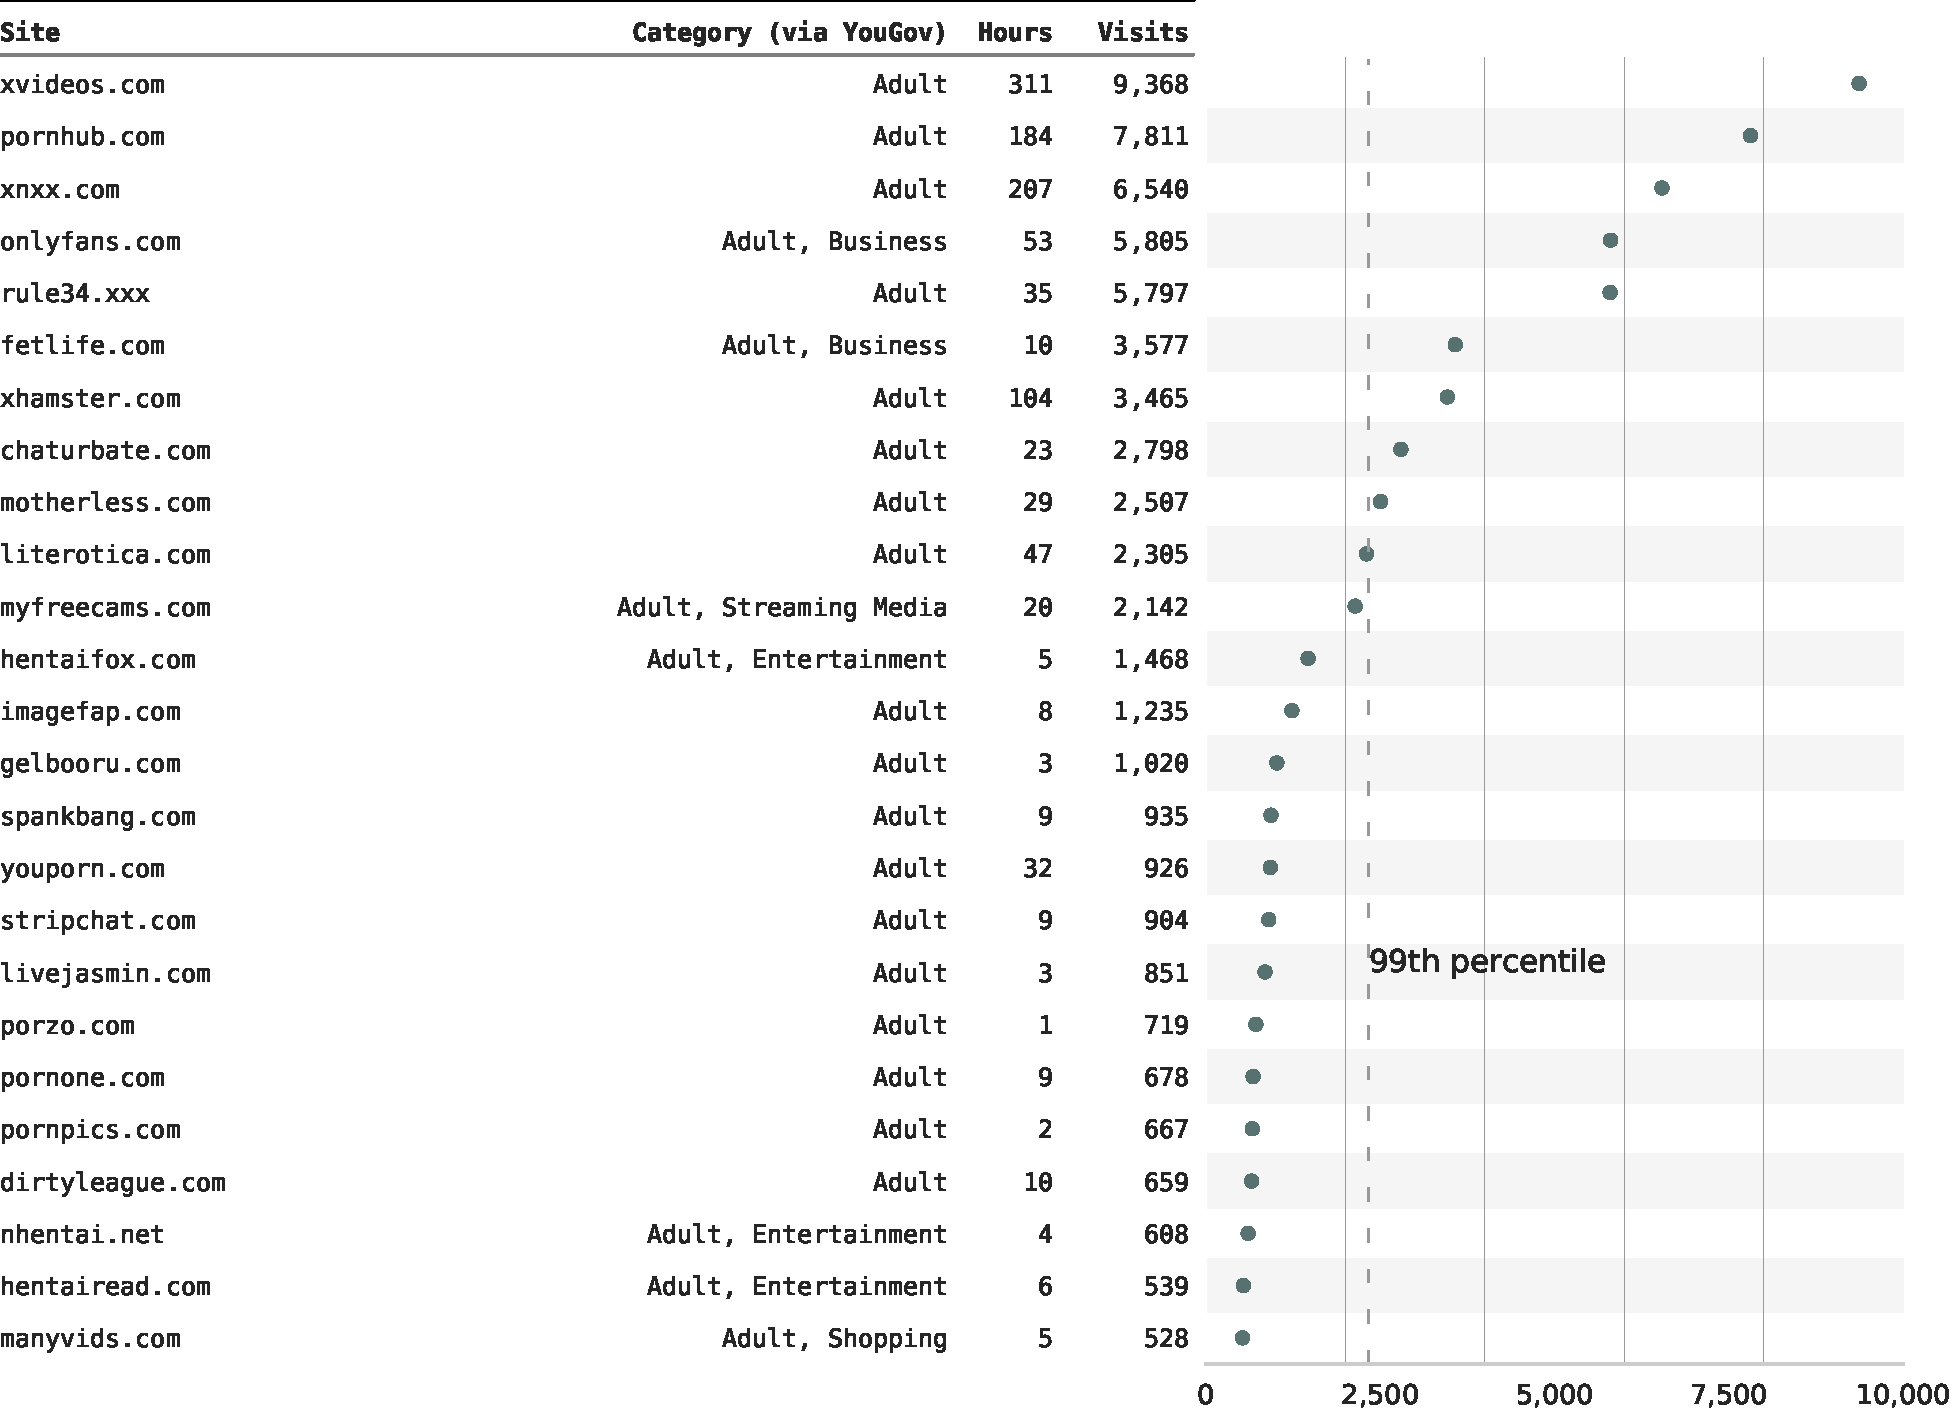
\includegraphics[scale=.75]{../figs/top_25_adultsites.pdf}
\label{fig:top25}
\end{figure}




\section{Consequence of Using Alternate Ways of Measuring Pornography}
\subsection{Keyword Classifier}
Our first classifier is based on just the domain name and domain suffix. In particular, we use a calibrated keyword classifier. The features of the model are whether any of the following keywords are present in the domain name:

\begin{quote}

cumshot, dildo, anal, adult, porn, mature, sex, xx, bbw, slut, whore, tits, titty, titties, pussy, sperm, gay, cheat, booty, ebony, asian, brazilian, fuck, cock, cunt, lesbian, shemale, boob, naughty, fatty, bitch, granny, jizz, faggot, horny, bukakke, bdsm, vagina, smut, x-rated, lusty, erotic, cunnilingus, blowjob, panty, hentai, latex, fetisch, fetish, erotik, bondage, naked, strip, teen, stocking, coitus, deprav, tube, perverse 

\end{quote}
\subsection{Machine Learning Classifier}

\section{Analysis of Visits}

\begin{figure}[h]
\centering
\caption{Distribution of Consumption of Pornography Online}
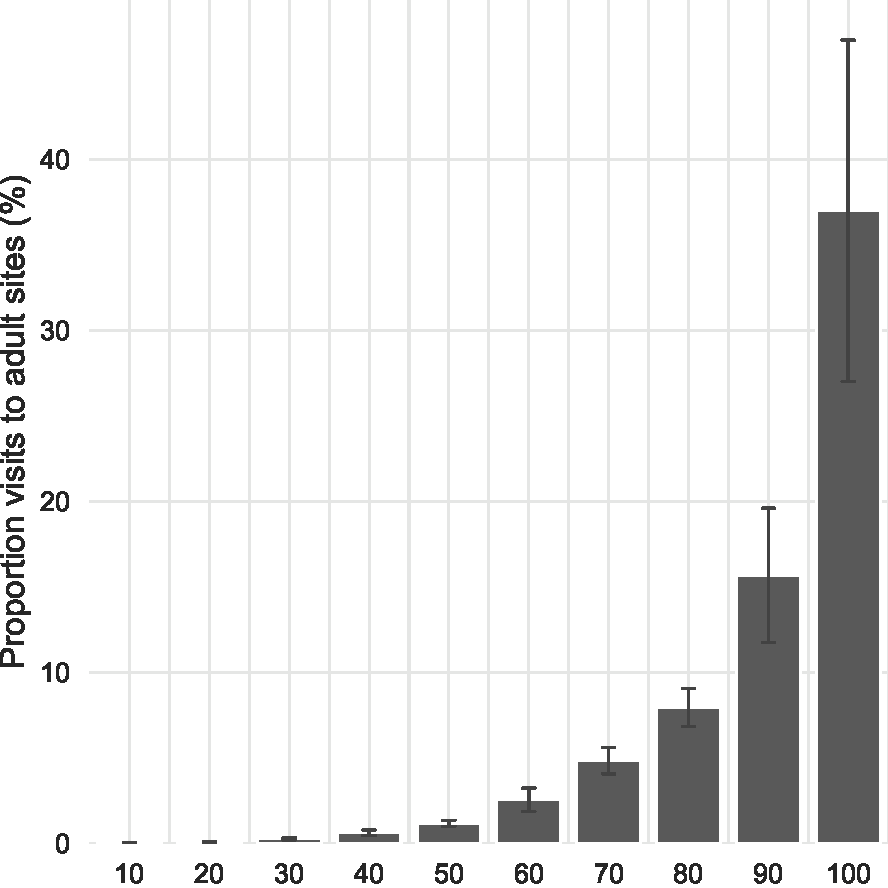
\includegraphics[scale=.75]{../figs/distribution_proportion_adultsites_visits.pdf}
\label{fig:distribution_visits}
\end{figure}

\begin{figure}[h]
\centering
\caption{Proportion of Visits to Pornographic Sites}
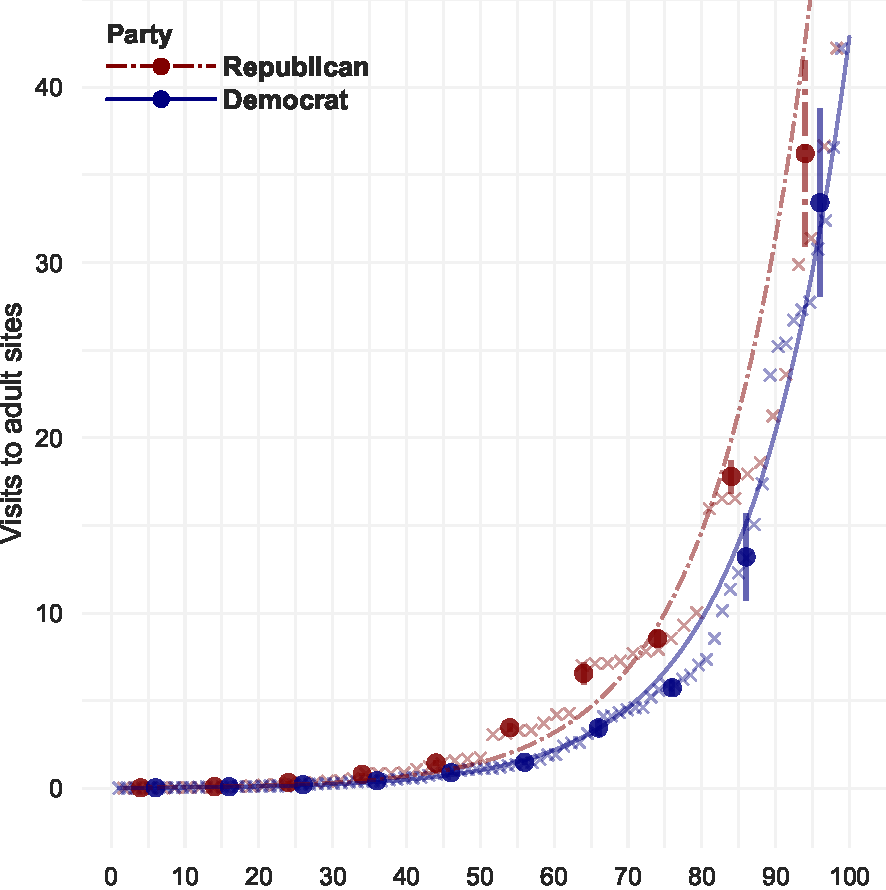
\includegraphics[scale=.75]{../figs/distribution_proportion_adultsites_visits_by_party.pdf}
\label{fig:distribution_prop_visits}
\end{figure}

\begin{figure}[h]
\centering
\caption{Distribution of Consumption of Pornography Online by Party}
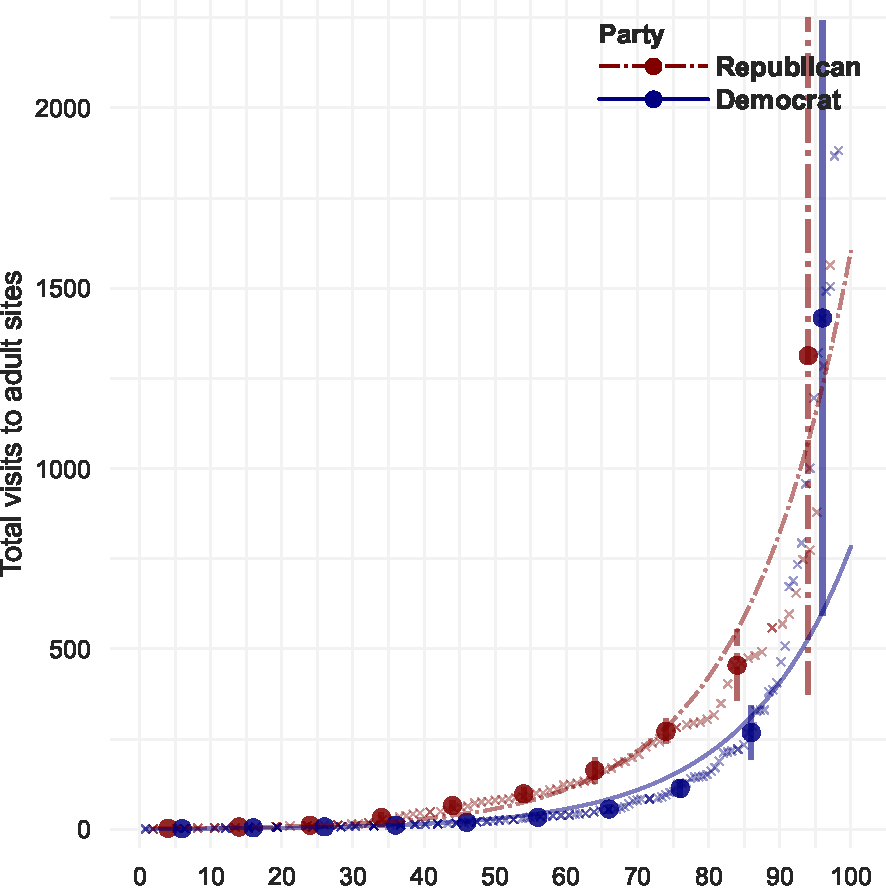
\includegraphics[scale=.75]{../figs/distribution_visits_to_adultsites_by_party.pdf}
\label{fig:distribution_visits_party}
\end{figure}

\end{document}
